\documentclass[tikz,border=4pt]{standalone}
\usepackage{fontspec}
\usepackage{xcolor}
\usetikzlibrary{arrows.meta,positioning,shapes.geometric}
\setmainfont{TeX Gyre Pagella}
\setsansfont{Lato}
\definecolor{bodyblue}{HTML}{DCE9F6}
\definecolor{accent}{HTML}{1A3F6E}
\begin{document}
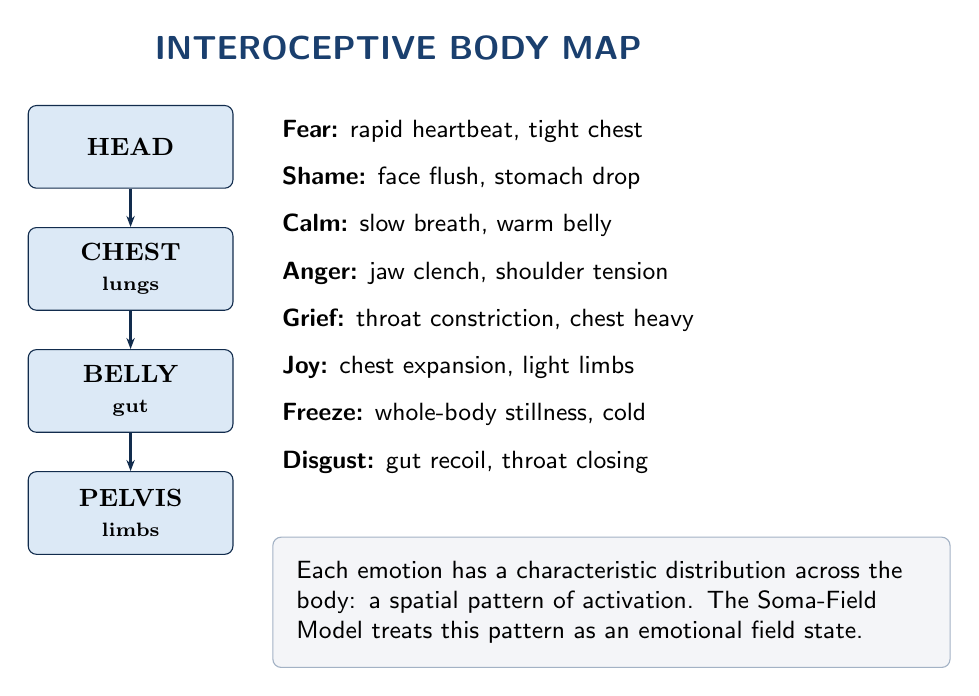
\begin{tikzpicture}[font=\sffamily,region/.style={rounded corners=3pt,draw=accent!70!black,fill=bodyblue,minimum width=2.6cm,minimum height=1.05cm,align=center,font=\small\bfseries},symptom/.style={font=\small\sffamily,anchor=west}]
  \node[font=\large\bfseries\sffamily,text=accent] at (4.8,5.7) {INTEROCEPTIVE BODY MAP};
  \node[region] (head) at (1.4,4.45) {HEAD};
  \node[region] (chest) at (1.4,2.9) {CHEST\\\scriptsize lungs};
  \node[region] (belly) at (1.4,1.35) {BELLY\\\scriptsize gut};
  \node[region] (pelvis) at (1.4,-.2) {PELVIS\\\scriptsize limbs};
  \draw[-{Stealth[length=4pt]},line width=.8pt,accent!70!black] (head) -- (chest);
  \draw[-{Stealth[length=4pt]},line width=.8pt,accent!70!black] (chest) -- (belly);
  \draw[-{Stealth[length=4pt]},line width=.8pt,accent!70!black] (belly) -- (pelvis);
  \node[symptom] at (3.2,4.65) {\textbf{Fear:} rapid heartbeat, tight chest};
  \node[symptom] at (3.2,4.05) {\textbf{Shame:} face flush, stomach drop};
  \node[symptom] at (3.2,3.45) {\textbf{Calm:} slow breath, warm belly};
  \node[symptom] at (3.2,2.85) {\textbf{Anger:} jaw clench, shoulder tension};
  \node[symptom] at (3.2,2.25) {\textbf{Grief:} throat constriction, chest heavy};
  \node[symptom] at (3.2,1.65) {\textbf{Joy:} chest expansion, light limbs};
  \node[symptom] at (3.2,1.05) {\textbf{Freeze:} whole-body stillness, cold};
  \node[symptom] at (3.2,.45) {\textbf{Disgust:} gut recoil, throat closing};
  \node[draw=accent!40,rounded corners=3pt,fill=accent!5,text width=8cm,align=left,font=\small\sffamily,anchor=north west,inner sep=3mm] at (3.2,-.5) {Each emotion has a characteristic distribution across the body: a spatial pattern of activation. The Soma-Field Model treats this pattern as an emotional field state.};
\end{tikzpicture}
\end{document}
